
\begin{slide}{Computational Paradigms}
 \begin{columns}
  \begin{column}{0.5\textwidth}
  \only<2, 6>{
  \begin{figure}
  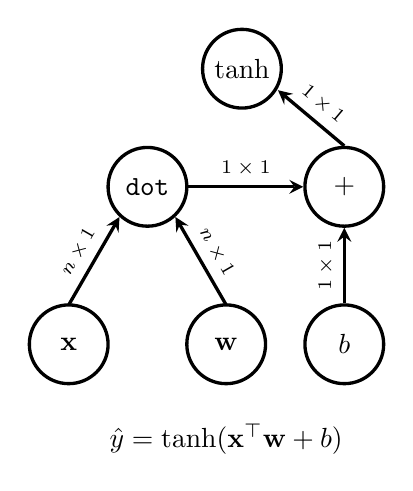
\begin{tikzpicture}
    % x^T w
    \draw [very thick] (1, 2) circle [radius=0.5cm] node {\texttt{dot}};

    % x and weights
    \draw [very thick] (0, 0) circle [radius=0.5cm] node {$\mathbf{x}$};
    \draw [very thick] (2, 0) circle [radius=0.5cm] node {$\mathbf{w}$};

    % Edges
    \draw [very thick, -stealth] (0, 0.5) -- ++(60:1.29)
          node [sloped, above, midway] {\scriptsize $n \times 1$};
    \draw [very thick, -stealth] (2, 0.5) -- ++(120:1.29)
          node [sloped, above, midway] {\scriptsize $n \times 1$};

    % Bias
    \draw [very thick] (3.5, 0) circle [radius=0.5cm] node {$b$};

    % z = (x^T w) + b
    \draw [very thick] (3.5, 2) circle [radius=0.5cm] node {$+$};


    % Edges
    \draw [very thick, -stealth] (3.5, 0.52) -- (3.5, 1.48)
          node [sloped, midway, above] {\scriptsize $1 \times 1$};
    \draw [very thick, -stealth] (1.52, 2) -- (2.98, 2)
          node [sloped, midway, above] {\scriptsize $1 \times 1$};

    % Sigmoid
    \draw [very thick] (2.2, 3.5) circle [radius=0.5] node {$\tanh$};

    % Edge
    \draw [very thick, -stealth] (3.5, 2.52) -- ++(140:1.1cm)
          node [sloped, midway, above] {\scriptsize $1 \times 1$};


    % Figure Label
    \draw (2, -1.2) node {$\hat{y} = \tanh(\mathbf{x}^\top \mathbf{w} + b)$};
  \end{tikzpicture}
  \end{figure}
  }
    \only<3>{
  \begin{figure}
  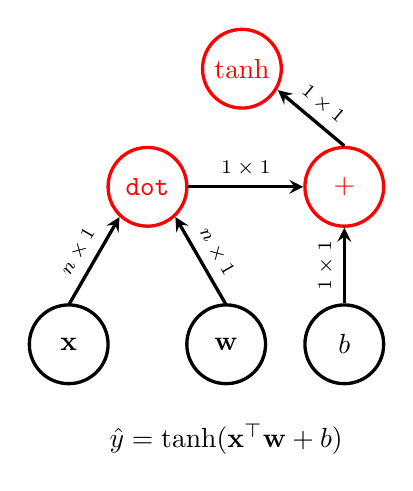
\begin{tikzpicture}
    % x^T w
    \draw [red, very thick] (1, 2) circle [radius=0.5cm] node {\texttt{dot}};

    % x and weights
    \draw [very thick] (0, 0) circle [radius=0.5cm] node {$\mathbf{x}$};
    \draw [very thick] (2, 0) circle [radius=0.5cm] node {$\mathbf{w}$};

    % Edges
    \draw [very thick, -stealth] (0, 0.5) -- ++(60:1.29)
          node [sloped, above, midway] {\scriptsize $n \times 1$};
    \draw [very thick, -stealth] (2, 0.5) -- ++(120:1.29)
          node [sloped, above, midway] {\scriptsize $n \times 1$};

    % Bias
    \draw [very thick] (3.5, 0) circle [radius=0.5cm] node {$b$};

    % z = (x^T w) + b
    \draw [red, very thick] (3.5, 2) circle [radius=0.5cm] node {$+$};


    % Edges
    \draw [very thick, -stealth] (3.5, 0.52) -- (3.5, 1.48)
          node [sloped, midway, above] {\scriptsize $1 \times 1$};
    \draw [very thick, -stealth] (1.52, 2) -- (2.98, 2)
          node [sloped, midway, above] {\scriptsize $1 \times 1$};

    % Sigmoid
    \draw [red, very thick] (2.2, 3.5) circle [radius=0.5] node {$\tanh$};

    % Edge
    \draw [very thick, -stealth] (3.5, 2.52) -- ++(140:1.1cm)
          node [sloped, midway, above] {\scriptsize $1 \times 1$};


    % Figure Label
    \draw (2, -1.2) node {$\hat{y} = \tanh(\mathbf{x}^\top \mathbf{w} + b)$};
  \end{tikzpicture}
  \end{figure}
  }
  \only<4>{
  \begin{figure}
  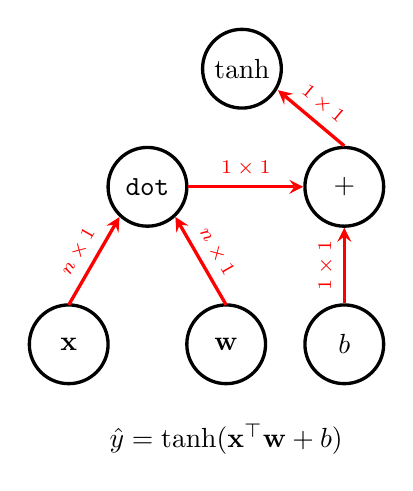
\begin{tikzpicture}
    % x^T w
    \draw [very thick] (1, 2) circle [radius=0.5cm] node {\texttt{dot}};

    % x and weights
    \draw [very thick] (0, 0) circle [radius=0.5cm] node {$\mathbf{x}$};
    \draw [very thick] (2, 0) circle [radius=0.5cm] node {$\mathbf{w}$};

    % Edges
    \draw [red, very thick, -stealth] (0, 0.5) -- ++(60:1.29)
          node [sloped, above, midway] {\scriptsize $n \times 1$};
    \draw [red, very thick, -stealth] (2, 0.5) -- ++(120:1.29)
          node [sloped, above, midway] {\scriptsize $n \times 1$};

    % Bias
    \draw [very thick] (3.5, 0) circle [radius=0.5cm] node {$b$};

    % z = (x^T w) + b
    \draw [very thick] (3.5, 2) circle [radius=0.5cm] node {$+$};


    % Edges
    \draw [red, very thick, -stealth] (3.5, 0.52) -- (3.5, 1.48)
          node [sloped, midway, above] {\scriptsize $1 \times 1$};
    \draw [red, very thick, -stealth] (1.52, 2) -- (2.98, 2)
          node [sloped, midway, above] {\scriptsize $1 \times 1$};

    % Sigmoid
    \draw [very thick] (2.2, 3.5) circle [radius=0.5] node {$\tanh$};

    % Edge
    \draw [red, very thick, -stealth] (3.5, 2.52) -- ++(140:1.1cm)
          node [sloped, midway, above] {\scriptsize $1 \times 1$};


    % Figure Label
    \draw (2, -1.2) node {$\hat{y} = \tanh(\mathbf{x}^\top \mathbf{w} + b)$};
  \end{tikzpicture}
  \end{figure}
  }
  \only<5>{
  \begin{figure}
  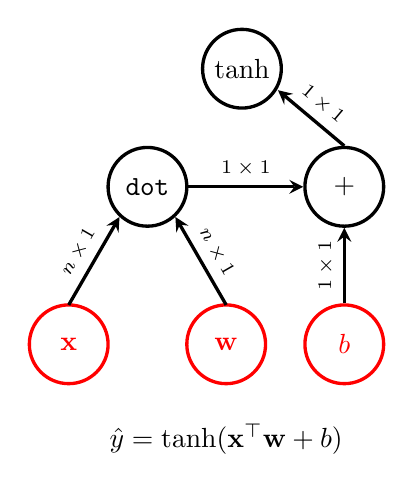
\begin{tikzpicture}
    % x^T w
    \draw [very thick] (1, 2) circle [radius=0.5cm] node {\texttt{dot}};

    % x and weights
    \draw [red, very thick] (0, 0) circle [radius=0.5cm] node {$\mathbf{x}$};
    \draw [red, very thick] (2, 0) circle [radius=0.5cm] node {$\mathbf{w}$};

    % Edges
    \draw [very thick, -stealth] (0, 0.5) -- ++(60:1.29)
          node [sloped, above, midway] {\scriptsize $n \times 1$};
    \draw [very thick, -stealth] (2, 0.5) -- ++(120:1.29)
          node [sloped, above, midway] {\scriptsize $n \times 1$};

    % Bias
    \draw [red, very thick] (3.5, 0) circle [radius=0.5cm] node {$b$};

    % z = (x^T w) + b
    \draw [very thick] (3.5, 2) circle [radius=0.5cm] node {$+$};


    % Edges
    \draw [very thick, -stealth] (3.5, 0.52) -- (3.5, 1.48)
          node [sloped, midway, above] {\scriptsize $1 \times 1$};
    \draw [very thick, -stealth] (1.52, 2) -- (2.98, 2)
          node [sloped, midway, above] {\scriptsize $1 \times 1$};

    % Sigmoid
    \draw [very thick] (2.2, 3.5) circle [radius=0.5] node {$\tanh$};

    % Edge
    \draw [very thick, -stealth] (3.5, 2.52) -- ++(140:1.1cm)
          node [sloped, midway, above] {\scriptsize $1 \times 1$};


    % Figure Label
    \draw (2, -1.2) node {$\hat{y} = \tanh(\mathbf{x}^\top \mathbf{w} + b)$};
  \end{tikzpicture}
  \end{figure}
  }
  \end{column}

  \begin{column}{0.5\textwidth}
  \vfill
  \vspace{0.7cm}
  \hspace{0.2cm}\pause \textbf{Computational Graphs}
  \vspace{0.2cm}
  \begin{enumerate}
    \item \pause Operations
    \item \pause Tensors
    \item \pause Variables
    \item \pause Sessions
  \end{enumerate}
  \end{column}
 \end{columns}
\end{slide}

%%% Local Variables:
%%% mode: latex
%%% TeX-master: "../presentation.tex"
%%% End: